\documentclass{beamer}

\usetheme[]{Rochester}
\usecolortheme{beaver}
\usepackage[latin1]{inputenc}
\usepackage{graphics}

\author{Will Webberley}
\date{Autumn 2014}
\institute[COMSC]{Cardiff School of Computer Science and Informatics}



\title{Design Patterns}
\subtitle{CM2101: Human-Computer Interaction}

\begin{document}

\frame{\titlepage}

\frame{
    \frametitle{Selective attention}
    Video
}

\frame{
    \frametitle{Selective attention: symptoms}
    \begin{itemize}
        \item If objects aren't central to task, they might not be noticed
        \item Even if staring right at the screen, may miss something if not obvious
        \item Important information may be missed
        \item Users may not be able to learn how to use a system
    \end{itemize}
}

\frame{
    \frametitle{Selective attention: causes}
    \begin{itemize}
        \item Human cognition
        \item Limitied ability to do more than one thing simultaneously
        \item Human working memory is a bottleneck for incoming information
        \item People often don't apply all of their focus to systems
        \item People are often doing other things at the same time
    \end{itemize}
}

\frame{
    \frametitle{Selective attention}
    \textbf{Users look at parts of the UI based on:}
    \vskip20pt
    \begin{itemize}
        \item \alert{Expectency} - where information is anticipated to be placed
        \item \alert{Relevance} - where relevant information/stimuli are
    \end{itemize}
    \vskip20pt
    Design interfaces to guide user attention.
}

\frame{
    \frametitle{Keeping user attention}
    \begin{itemize}
        \item Reduce distraction \& attention-competing elements
        \begin{itemize}
            \item Make task-specific information stand out
            \item Use attention redirection to improve task performance (e.g. animations)
        \end{itemize}
        \item Tasks should be presented serially, not in parallel, where possible
        \begin{itemize}
            \item Sometimes, users can switch (e.g. when waiting for a download or for programs to run)
        \end{itemize}
        \item Reduce memory load (\alert{Recognition vs recall})
        \begin{itemize}
            \item Follow guidelines for platform
            \item Adhere to general principles and standards
            \item Don't overload user
            \item Closure: give feedback for tasks
        \end{itemize}
    \end{itemize}
}

\frame{
    \frametitle{Keeping user attention}
    \begin{center}
        \alert{Design patterns} help address these areas
    \end{center}
}

\frame{
    \frametitle{Design patterns in software}
    \begin{itemize}
        \item General \alert{reusable solution} to a common problem
        \item It is a \alert{`template'}, and thus not a finished design
        \item Used in \alert{many situations}, domains, and contexts
        \item Different patterns can be used together 
        \item Different patterns can be used for different purposes
    \end{itemize}
}

\frame{
    \frametitle{Design patterns in software}
    \textbf{Example software design patterns:}
    \begin{itemize}
        \item Factory method
        \item Singleton
        \item Adapter
        \item Decorator
        \item Observer \& publish/subscribe
        \item Thread locking
        \item Thread pooling
    \end{itemize}
}

\frame{
    \frametitle{Design patterns for interface design}
    \begin{itemize}
        \item Same as for software
        \begin{itemize}
            \item \alert{Reusable solution} to a common problem
            \item \alert{`Template'}, and thus not a finished design
            \item Used in \alert{many situations}, domains, and contexts
            \item ...
        \end{itemize}
        \item Essentially a reusable `layout' of the UI 
        \item Reusable across apps (external consistency)
        \item Reusable in screens in apps (internal consistency)
        \item Each pattern has a predefined `problem' it solves
    \end{itemize}
}

\frame{
    \frametitle{Types of UI design patterns}
    \textbf{Design patterns fall into 3 main categories}
    \vskip20pt
    \begin{itemize}
        \item \alert{Structural}
        \begin{itemize}
            \item Organising page layout
            \item Address aesthetics
            \item Show info in a more easy way to understand (gulf of evaluation)
        \end{itemize}
        \item \alert{Functional}
        \begin{itemize}
            \item Doing things (e.g. buttons and controls)
            \item Getting input from users (e.g. forms)
        \end{itemize}
        \item \alert{Navigational}
        \begin{itemize}
            \item Moving around an interface
            \item Navigating between screens
        \end{itemize}
    \end{itemize}
}

\frame{
    \frametitle{Design pattern: `Master/detail'}
    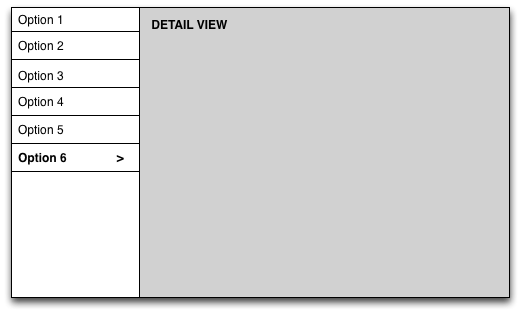
\includegraphics[width=\textwidth]{media/master_detail_1.png}
}

\frame{
    \frametitle{Design pattern: `Master/detail' example}
    \begin{center}
        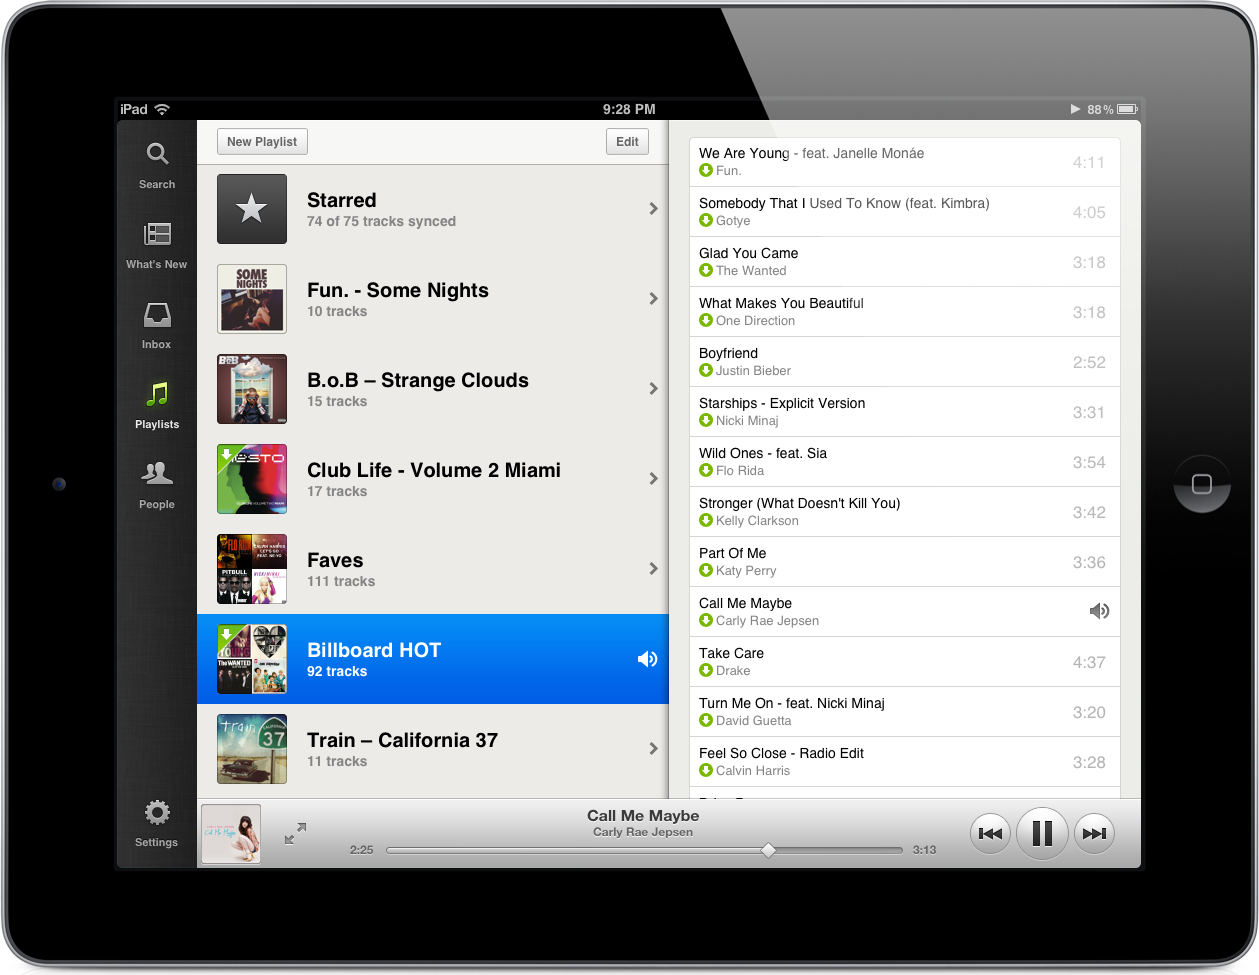
\includegraphics[width=.8\textwidth]{media/master_detail_2.png}
    \end{center}
}

\frame{
    \frametitle{Design pattern: `Column browse'}
    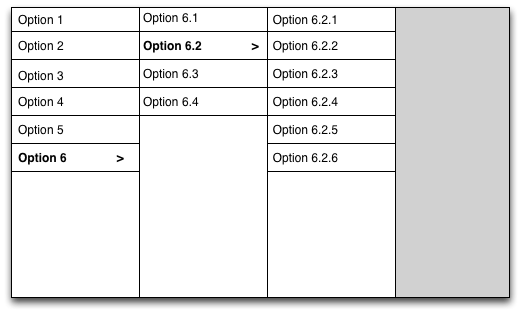
\includegraphics[width=\textwidth]{media/columns_1.png}
}

\frame{
    \frametitle{Design pattern: `Column browse' example}
    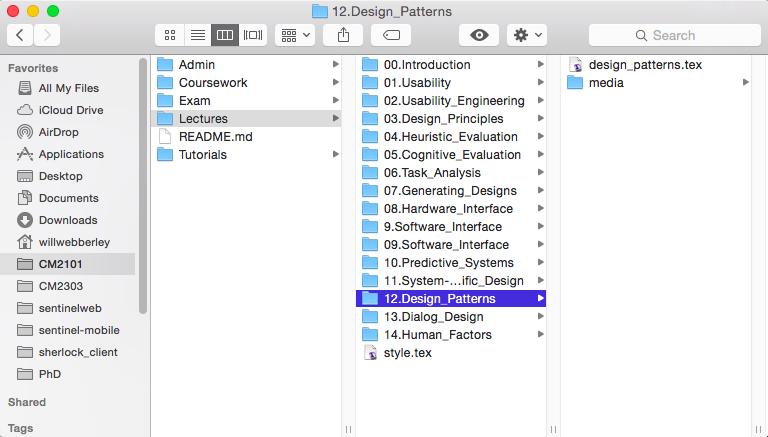
\includegraphics[width=\textwidth]{media/columns_2.png}
}

\frame{
    \frametitle{Design pattern: `Search/results'}
    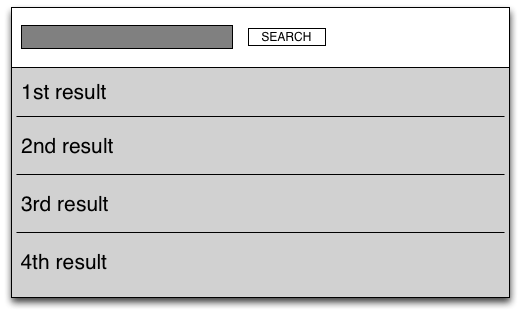
\includegraphics[width=\textwidth]{media/search_1.png}
}

\frame{
    \frametitle{Design pattern: `Search/results' example}
    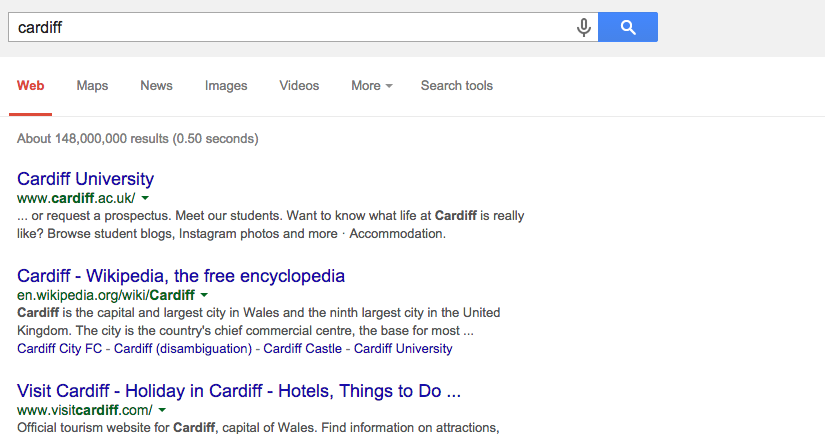
\includegraphics[width=\textwidth]{media/search_2.png}
}

\frame{
    \frametitle{Design pattern: `Filter/results'}
    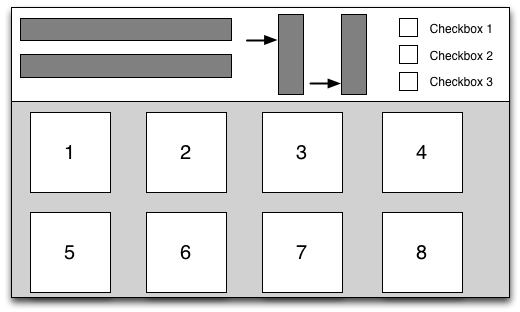
\includegraphics[width=\textwidth]{media/filter_1.png}
}

\frame{
    \frametitle{Design pattern: `Filter/results' example}
    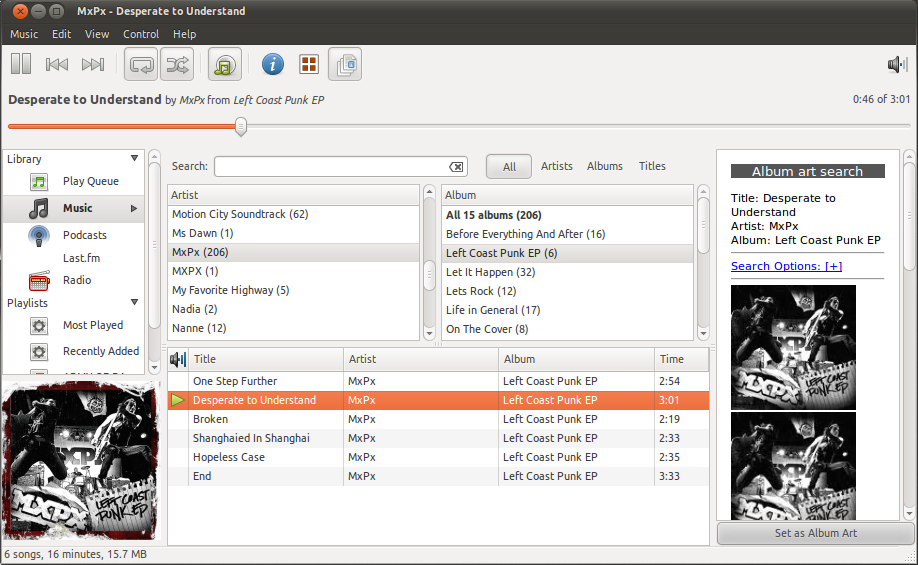
\includegraphics[width=\textwidth]{media/filter_2.png}
}

\frame{
    \frametitle{Design pattern: `Form'}
    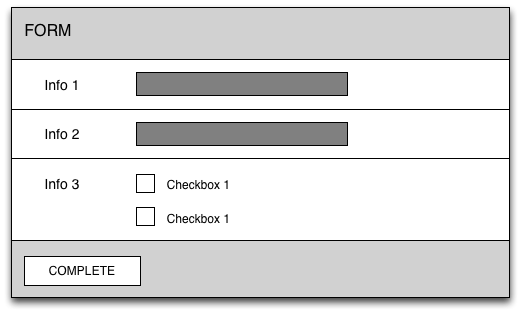
\includegraphics[width=\textwidth]{media/form_1.png}
}

\frame{
    \frametitle{Design pattern: `Form' example}
    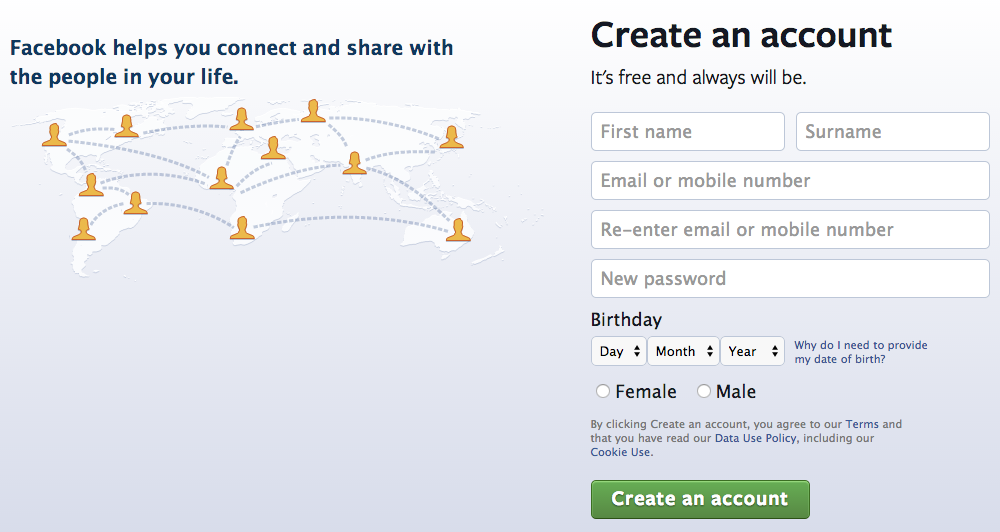
\includegraphics[width=\textwidth]{media/form_2.png}
}

\frame{
    \frametitle{Design pattern: `Palette/canvas'}
    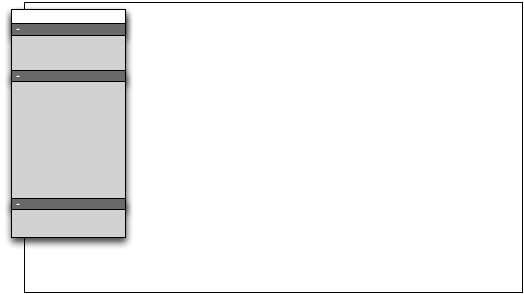
\includegraphics[width=\textwidth]{media/palette_1.png}
}

\frame{
    \frametitle{Design pattern: `Palette/canvas' example}
    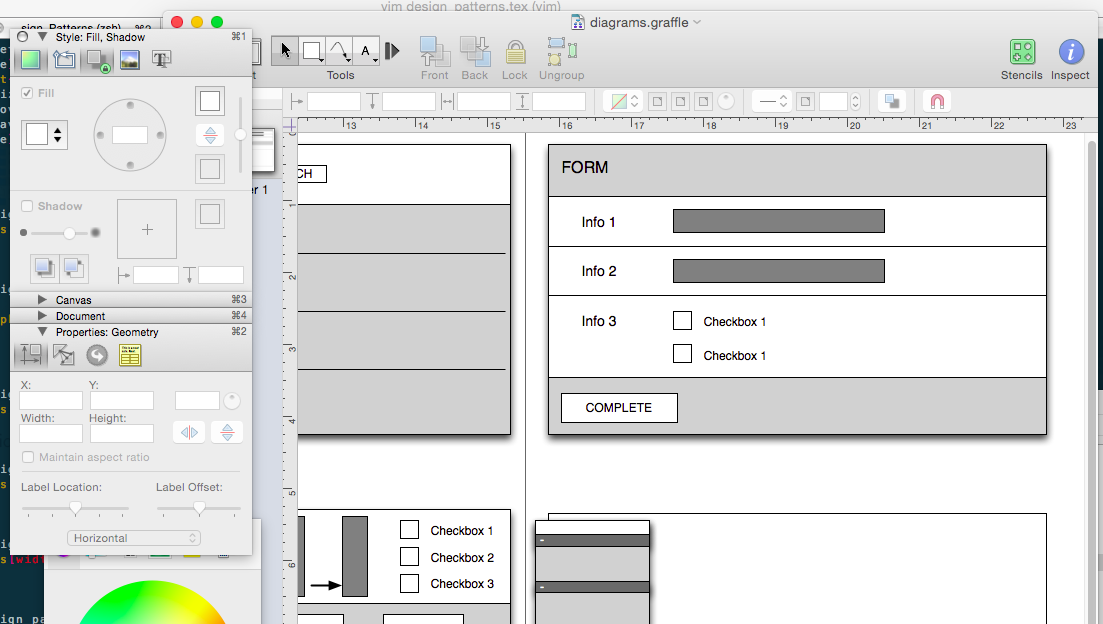
\includegraphics[width=\textwidth]{media/palette_2.png}
}

\frame{
    \frametitle{Design pattern: `Wizard'}
    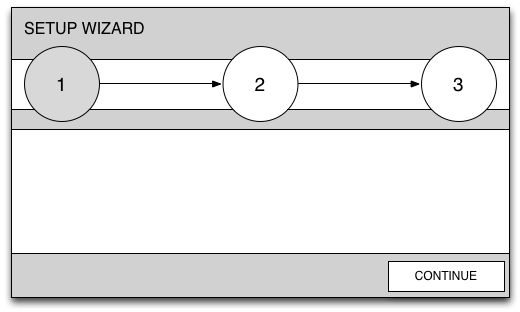
\includegraphics[width=\textwidth]{media/wizard_1.png}
}

\frame{
    \frametitle{Design pattern: `Wizard' example}
    \begin{center}
        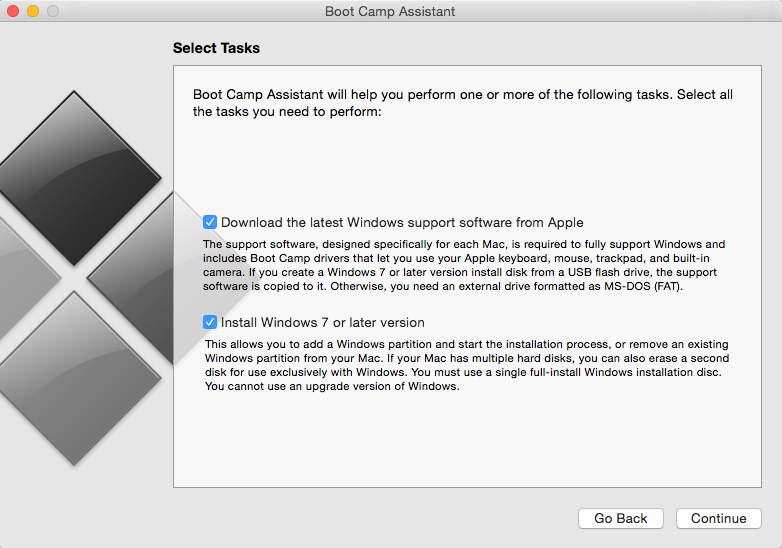
\includegraphics[width=.9\textwidth]{media/wizard_2.png}
    \end{center}
}

\frame{
    \frametitle{Design pattern: `Dashboard'}
    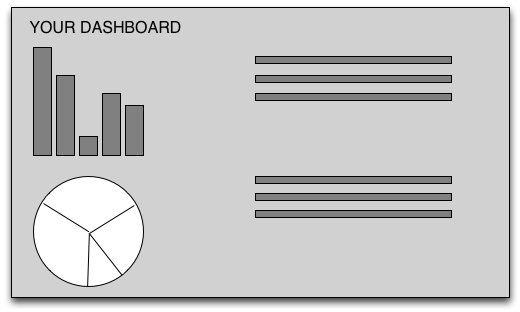
\includegraphics[width=\textwidth]{media/dashboard_1.png}
}

\frame{
    \frametitle{Design pattern: `Dashboard' example}
    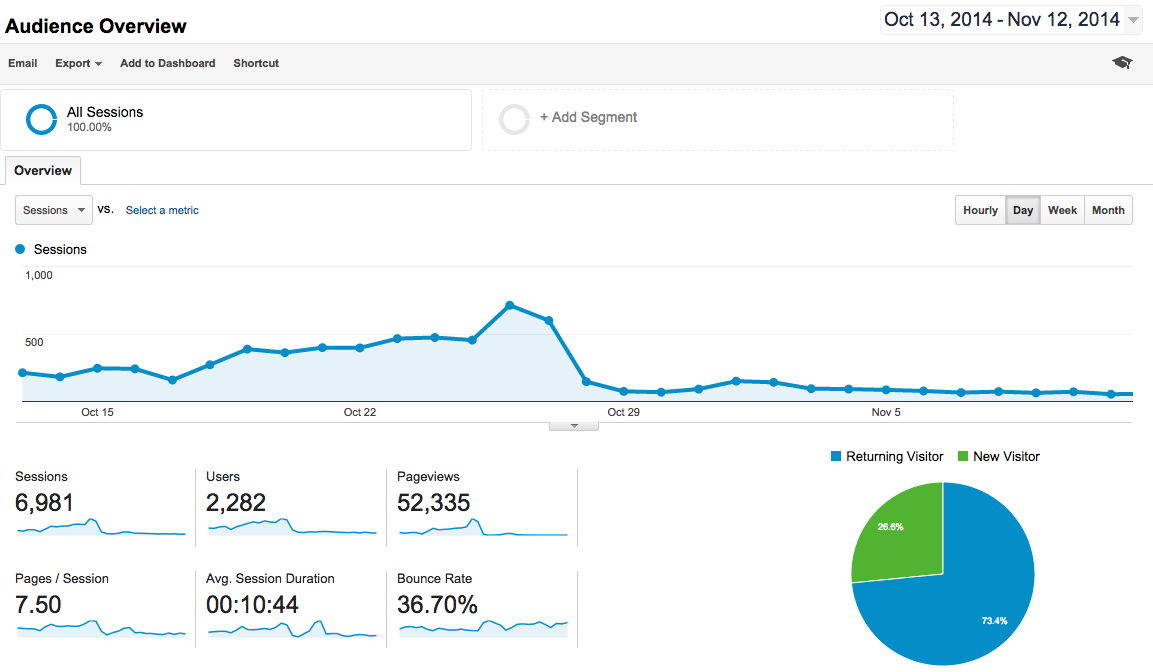
\includegraphics[width=\textwidth]{media/dashboard_2.png}
}

\frame{
    \frametitle{Design pattern: `Grid of Equals'}
    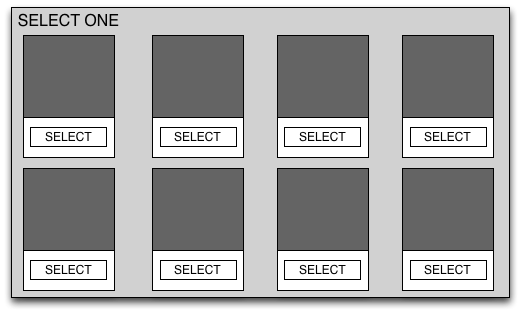
\includegraphics[width=\textwidth]{media/grid_1.png}
}

\frame{
    \frametitle{Design pattern: `Grid of Equals' example}
    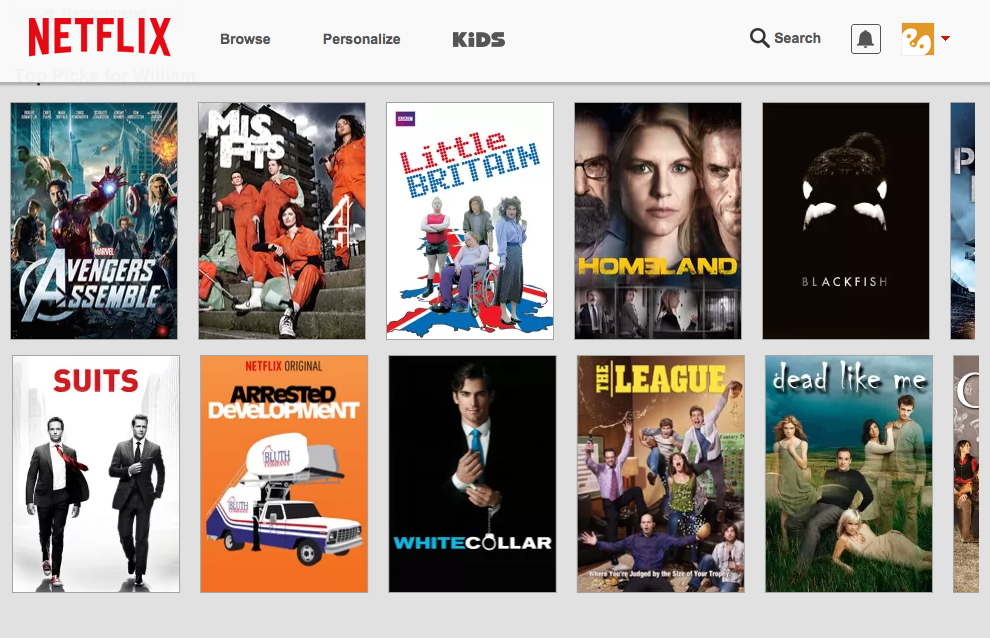
\includegraphics[width=\textwidth]{media/grid_2.png}
}

\frame{
    \frametitle{Design patterns}
    \begin{center}
        + many more
    \end{center}
    \vskip20pt
    Some come under different names or slightly different structures
}

\frame{
    \frametitle{Using design patterns}
    \begin{itemize}
        \item Identify what information you want to display or harvest
        \vskip15pt
        \item Is the information \alert{visual}? (grid of equals)
        \item Is the information \alert{searchable}? (search or filter)
        \item Is the information data that needs to be \alert{rendered}? (dashboard)
        \item Do you need to \alert{collect} information? (form)
        \item Do you need to \alert{configure} a system? (wizard) 
    \end{itemize}    
    \vskip20pt
    Once you know what information needs to be displayed or collected, it's easier to find a useful pattern.
}

\frame{
    \frametitle{Using design patterns}
    Usually, ready-made patterns available for use or download.
    \begin{itemize}
        \item Slideshows
        \item Galleries
        \item Product lists
        \item Forms
        \item Use of `Fragments' on Android
    \end{itemize}
    \vskip10pt
    Most pre-built `patterns' implement a single (or combination of) standard design pattern
}

\frame{
    \frametitle{Using design patterns}
    Implement your own or find pre-built ones on the web:
    \begin{itemize}
        \item ui-patterns.com
        \item pttrns.com
        \item welie.com/patterns
        \vskip20pt
        \item ... (search the web for more)
    \end{itemize}
}

\frame{
     \frametitle{Revision questions}
     \begin{enumerate}
        \item What is meant by the term `selective attention'?
        \item Why does selective attention occur?
        \item How can the problem of selective attention be addressed?
        \item What is meant by the term `design pattern' in general?
        \item What are the three main types of interface design pattern?
        \item Describe the `master/detail' design pattern.
        \item How would one decide on which design pattern to use?
     \end{enumerate}
}

\frame{
    \frametitle{Summary}
    \begin{itemize}
        \item Selective attention: the problem
        \item Selective attention: solution
        \item Design patterns in software
        \item Design patterns in user interfaces
        \item Examples of interface design patterns
        \item Using and implementing interface design patterns
    \end{itemize}
}    

\end{document}
